\documentclass[10pt,a4paper]{letter}
\usepackage[utf8]{inputenc}
\usepackage[portuguese]{babel}
\usepackage[T1]{fontenc}
\usepackage{amsmath}
\usepackage{amsfonts}
\usepackage{amssymb}
\usepackage[left=2cm,right=2cm,top=2cm,bottom=2cm]{geometry}
\author{Pedro Henrique Lima Carvalho}
\usepackage{graphicx}
\graphicspath{ {./images/} }
\newenvironment{resposta}{%
  \par%
  \medskip
  \leftskip=4em%
  \noindent\ignorespaces}{%
  \par\medskip}
  

\begin{document} 
\noindent
PUC Minas - Ciência da Computação \\
Coração Eucarístico \\
PAA - Manhã \\
Pedro Henrique Lima Carvalho 
\par\noindent

Seja $A = {(x_{i},\; y_{i}\;|\; i \in [1, n]}$ um conjunto de $n$ pontos. Resolva o problema de encontrar o par de pontos mais próximos no plano, considerando três diferentes soluções com os seguintes custos computacionais:
\par 

a) \textbf{O}($n^{2}$)
\begin{resposta}
Para uma solução com complexidade \textbf{O}($n^{2}$), utiliza-se um algoritmo de força bruta. Ou seja, calcula-se todas as distâncias entre todos os pares de pontos e seleciona os dois pares cuja distância seja a menor. 
\par
Considerando que o problema tenha $n$ pontos, é necessário calcular $\binom{n}{2}$ distâncias. Ou seja:
\[\frac{n!}{(n-2)!*2!} = \frac{n(n-1)}{2} = \frac{n^2-n}{2} = O(n^2) \]
\end{resposta}

\par b) \textbf{O}($nlog^{2}n$)
\begin{resposta}
Já para uma solução com complexidade inferior à obtida através do algoritmo de força bruta, faça-se necessária a utilização de outra estratégia. No caso, adota-se uma estratégia de divisão e conquista.\\ Primeiramente, os $n$ pontos são ordenados pelo eixo $X$, utilizando um algoritmo de complexidade $O(nLogn)$. No caso, foi escolhido o algoritmo \textit{heapSort}.
\par 
Uma vez que os pontos estajam ordenados, entra a estratégia de divisão. O plano é dividido por uma reta $L$ em dois, $Q$ e $R$, calculando-se a menor distância de cada metade. Essa estratégia é aplicada recusivamente, até o caso base(três ou menos pontos). Havendo três ou menos pontos, a menor distância é calculada por for força bruta. Assim, o problema é sempre divido em dois, totalizando $Log(n)$ níveis de recursão.
\par 
No retorno da recursão é feita a combinação dos resultados de cada lado, selecionando o par de pontos de menor distância. Essa menor distância chamaremos de $\delta$. 
\begin{center}
\par
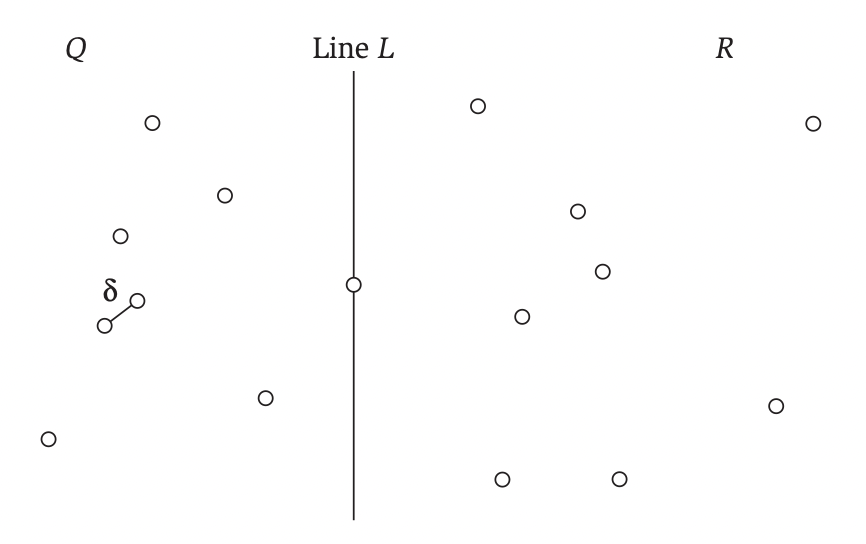
\includegraphics[width=.6\textwidth]{divisao}\\
Algorithm design / Jon Kleinberg, Éva Tardos. 1st ed.
\end{center}
\newpage 
 No entanto, é possível que a distância entre um ponto de $Q$ e um ponto de $R$ seja menor que $\delta$. E como só foi calculada a menor distância de cada metade, essa distância está sendo desconsiderada.
\begin{center}
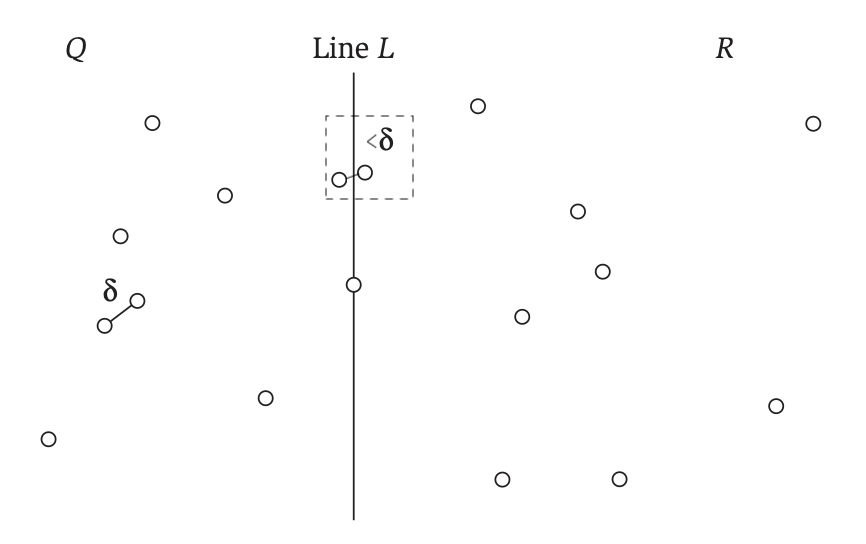
\includegraphics[width=.6\textwidth]{delta}\\
\end{center}
Para isso, também é necessário calcular a distância entre pontos de $Q$ e de $R$ que estejam a uma distância $\delta$ de $L$. Porém, essa distância $\delta$ pode ser o próprio tamanho de $Q$ ou $R$, o que implicaria em uma complexidade $O(n^2)$.
\par 
No entanto, como a menor distância entre dois pontos que estejam no mesmo lado é $\delta$, ao dividirmos a faixa entre $L-\delta$ e $L+\delta$ em quadrados de lado $\delta/2$, temos certeza de que há apenas um ponto em cada quadrado.

\begin{center}
\par
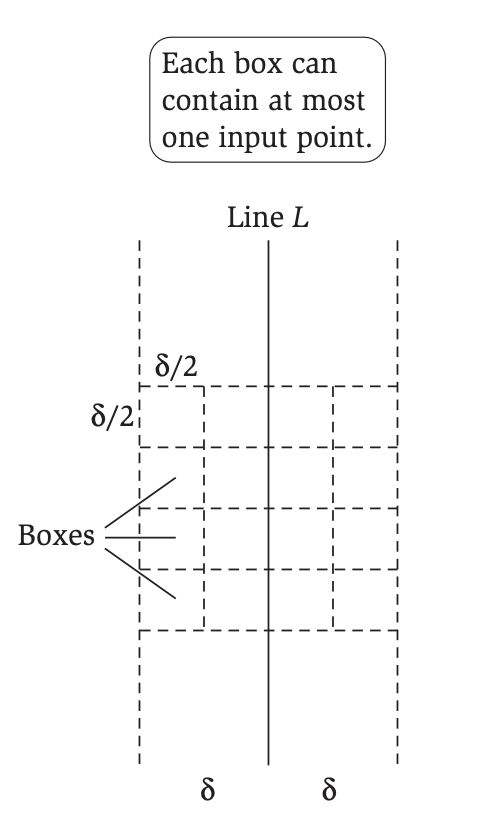
\includegraphics[width=.3\textwidth]{boxes}\\
Algorithm design / Jon Kleinberg, Éva Tardos. 1st ed.
\end{center}

Logo, ordenando esses pontos pelo eixo $Y$, e começando do menor para o maior, para cada ponto, basta calcular sua distância para no máximo sete pontos. Assim, essa parte do algoritmo tem complexidade $O(nLogn)$ para a ordenação e $O(n)$ para o cálculo das distâncias, vez que para cada ponto calcula-se um número constante de distâncias.
\par 
Com dito acima, ao dividirmo o problema pela metade, temos $Log(n)$ níveis de recursão, sendo que, em cada nível, a operação de maior complexidade é a ordenanação pelo eixo $Y$ dos pontos na faixa entre $L-\delta$ e $L+\delta$.
\par 
Assim, a complexidade total do algoritmo é $O(nLog^2n)$.

\end{resposta}

\newpage
\par c) \textbf{O}($nlogn$)

\par 
\begin{resposta}
Essa solução, na realidade, utliza praticamente o mesmo algoritmo da solução $O(nLog^2n)$. A única otimização feita é a criação, no começo do algoritmo, de uma segunda lista dos pontos, ordenada pelo eixo $Y$. Tanto a lista ordenada pelo eixo $X$, quanto a ordenada pelo eixo $Y$, são passadas para cada recursão, evitando que seja necessária nova ordenação em cada chamada.
\par 
Assim, ao invés de termos $Log(n)$ níveis de recursão, cada um realizando ordenações com custo de $O(nLogn)$, temos em cada nível uma varredura da lista ordenada por $Y$ a um custo $O(n)$.
\par 
Portanto, o algoritmo todo tem uma complexidade de $O(nLogn)$.
\end{resposta}
\end{document}